\documentclass[]{article}
\usepackage{lmodern}
\usepackage{amssymb,amsmath}
\usepackage{ifxetex,ifluatex}
\usepackage{fixltx2e} % provides \textsubscript
\ifnum 0\ifxetex 1\fi\ifluatex 1\fi=0 % if pdftex
  \usepackage[T1]{fontenc}
  \usepackage[utf8]{inputenc}
\else % if luatex or xelatex
  \ifxetex
    \usepackage{mathspec}
  \else
    \usepackage{fontspec}
  \fi
  \defaultfontfeatures{Ligatures=TeX,Scale=MatchLowercase}
\fi
% use upquote if available, for straight quotes in verbatim environments
\IfFileExists{upquote.sty}{\usepackage{upquote}}{}
% use microtype if available
\IfFileExists{microtype.sty}{%
\usepackage{microtype}
\UseMicrotypeSet[protrusion]{basicmath} % disable protrusion for tt fonts
}{}
\usepackage[margin=1in]{geometry}
\usepackage{hyperref}
\hypersetup{unicode=true,
            pdftitle={206 HW 5},
            pdfauthor={Joslyn Fritz},
            pdfborder={0 0 0},
            breaklinks=true}
\urlstyle{same}  % don't use monospace font for urls
\usepackage{graphicx,grffile}
\makeatletter
\def\maxwidth{\ifdim\Gin@nat@width>\linewidth\linewidth\else\Gin@nat@width\fi}
\def\maxheight{\ifdim\Gin@nat@height>\textheight\textheight\else\Gin@nat@height\fi}
\makeatother
% Scale images if necessary, so that they will not overflow the page
% margins by default, and it is still possible to overwrite the defaults
% using explicit options in \includegraphics[width, height, ...]{}
\setkeys{Gin}{width=\maxwidth,height=\maxheight,keepaspectratio}
\IfFileExists{parskip.sty}{%
\usepackage{parskip}
}{% else
\setlength{\parindent}{0pt}
\setlength{\parskip}{6pt plus 2pt minus 1pt}
}
\setlength{\emergencystretch}{3em}  % prevent overfull lines
\providecommand{\tightlist}{%
  \setlength{\itemsep}{0pt}\setlength{\parskip}{0pt}}
\setcounter{secnumdepth}{0}
% Redefines (sub)paragraphs to behave more like sections
\ifx\paragraph\undefined\else
\let\oldparagraph\paragraph
\renewcommand{\paragraph}[1]{\oldparagraph{#1}\mbox{}}
\fi
\ifx\subparagraph\undefined\else
\let\oldsubparagraph\subparagraph
\renewcommand{\subparagraph}[1]{\oldsubparagraph{#1}\mbox{}}
\fi

%%% Use protect on footnotes to avoid problems with footnotes in titles
\let\rmarkdownfootnote\footnote%
\def\footnote{\protect\rmarkdownfootnote}

%%% Change title format to be more compact
\usepackage{titling}

% Create subtitle command for use in maketitle
\newcommand{\subtitle}[1]{
  \posttitle{
    \begin{center}\large#1\end{center}
    }
}

\setlength{\droptitle}{-2em}

  \title{206 HW 5}
    \pretitle{\vspace{\droptitle}\centering\huge}
  \posttitle{\par}
    \author{Joslyn Fritz}
    \preauthor{\centering\large\emph}
  \postauthor{\par}
      \predate{\centering\large\emph}
  \postdate{\par}
    \date{11/28/2018}

\usepackage{booktabs}
\usepackage{longtable}
\usepackage{array}
\usepackage{multirow}
\usepackage[table]{xcolor}
\usepackage{wrapfig}
\usepackage{float}
\usepackage{colortbl}
\usepackage{pdflscape}
\usepackage{tabu}
\usepackage{threeparttable}
\usepackage{threeparttablex}
\usepackage[normalem]{ulem}
\usepackage{makecell}

\begin{document}
\maketitle

\paragraph{1. Compare trends in graduate enrollment
(1967-2015)}\label{compare-trends-in-graduate-enrollment-1967-2015}

Male: t(47) = 16.61, p \textless{} 0.001. Reject the null. Correlation =
0.92, which is a strong positive correlation.

Year significantly predicts male graduate school enrollment (\emph{b} =
-17112153, t(47) = 16.61, \emph{p} \textless{} 0.001) with a strong
positive correlation between the two (Pearson's \emph{r} = 0.92). The
overall model (Total gradute male enrollment = 9060(year) - 17112153)
explains a significant amount of variance in male enrollment (F(1,47) =
276, \emph{p} \textless{} 0.001, R\textsuperscript{2} = 0.85).

Female: t(47) = 51.66, p \textless{} 0.001. Reject the null. Correlation
= 0.99, which is a strong positive correlation.

Year significantly predicts female graduate school enrollment (\emph{b}
= -17112153, t(47) = 16.61, \emph{p} \textless{} 0.001) with a strong
positive correlation between the two (Pearson's \emph{r} = 0.92). The
overall model (Total gradute female enrollment = 30126(year) - 58955502)
explains a significant amount of variance in male enrollment (F(1,47) =
2669, \emph{p} \textless{} 0.001, R\textsuperscript{2} = 0.98).

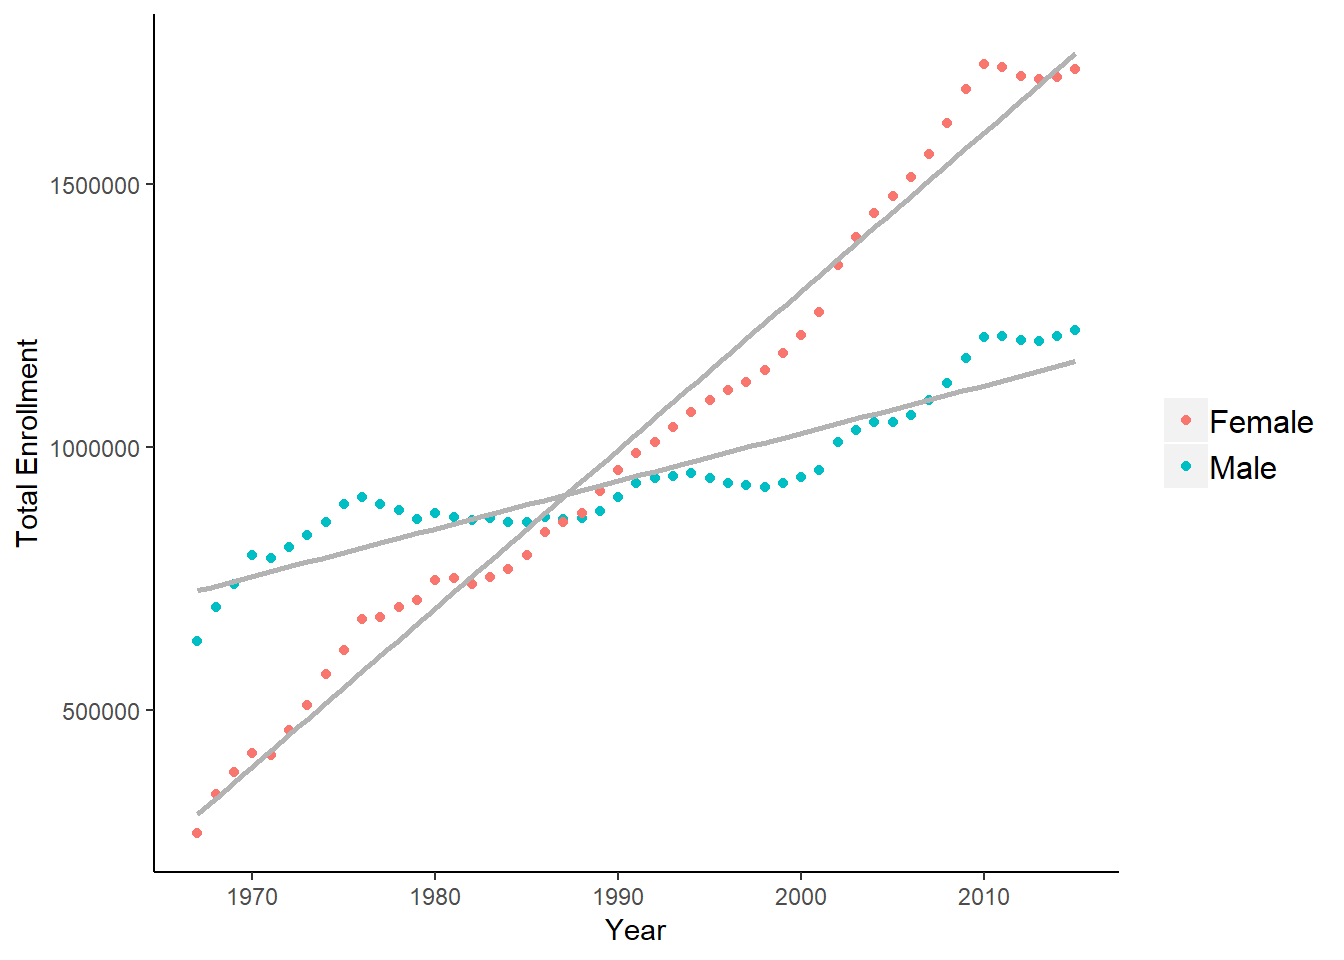
\includegraphics{206_HW_5_files/figure-latex/unnamed-chunk-5-1.pdf}

\paragraph{2. Shifts in Phd recipients by field of study (1985, 2000,
2015)}\label{shifts-in-phd-recipients-by-field-of-study-1985-2000-2015}

number of female phd recipients per field differed significantly between
1985 (n = ) and 2000 (n = ) and 2015 (n =) (\(\chi^2\)\{6\} =
\ldots{}.., p \textless{} 0.001). Notably, \ldots{}.

\begin{table}

\caption{\label{tab:unnamed-chunk-7}**Table 1. Proportions of female recipients who earned a Phd in 1985, 2000 and 2015.**}
\centering
\begin{tabular}[t]{>{\bfseries\raggedright\arraybackslash}p{15em}|>{\raggedleft\arraybackslash}p{15em}|>{\raggedleft\arraybackslash}p{15em}|r}
\hline
  & 1985 & 2000 & 2015\\
\hline
Education & 0.31 & 0.37 & 0.31\\
\hline
Engineering & 0.06 & 0.25 & 0.69\\
\hline
Humanities \& Art & 0.20 & 0.39 & 0.41\\
\hline
Physical Earth Sciences & 0.16 & 0.29 & 0.56\\
\hline
\end{tabular}
\end{table}

\paragraph{3. Male and female salaries for starting postdoc and other
positions
(2015)}\label{male-and-female-salaries-for-starting-postdoc-and-other-positions-2015}

There was no significant difference in median salary for male and female
starting postdoc positions (W = 180, p = 0.867, alpha = 0.05)

There was no significant difference in median salary for male and female
starting postdoc positions (W = 88.5, p = 0.329, alpha = 0.05)

\paragraph{4. Exploring academic salaries for professors in U.S.
colleges}\label{exploring-academic-salaries-for-professors-in-u.s.-colleges}


\end{document}
